\documentclass[aspectratio=169, 9pt]{beamer}

% 这是一个自定义的武汉大学数学与统计学院2021本科毕业答辩模板

%%%%%%%%%%%%%%%%%%%%%%%%%%%%%%%%%%%%%%%%%%%%%%%%%%%%%%%%%%%%%%%%%%%%%%%%%%%%%%%%%%
%   不要删除下列PACKAGE,但可以根据需要再添加PACKAGE
\usetheme{Warsaw}
\usecolortheme{whale}   %主题和颜色的选取参考
\usepackage[style=verbose]{biblatex} 
% 引文支持
\usepackage{filecontents}
\addbibresource{bibliography.bib}
\usepackage{tikz}
\usepackage{times}
\usepackage{hyperref}
\usepackage{graphicx} 
% 图支持
\usepackage{booktabs} 
% 表格支持
\usepackage{amsmath}
\usepackage{amsfonts}
\usepackage{amssymb}
\usepackage{subcaption}
\usepackage{siunitx} 
\usepackage{ctex}
\addtobeamertemplate{block begin}{}{\justifying}
\setbeamertemplate{section in toc}[sections numbered] 
% 创建目录
\setbeamertemplate{caption}[numbered] % 注释编号
\def\mathfamilydefault{\rmdefault} % 注释该行获得SANS风格的公式
\setsansfont{Times New Roman} % 默认英文为TimesNewRoman
\setbeamerfont{headline}{size=\tiny}
% 修改导航栏
\setbeamerfont{title}{size=\huge}
% 修改标题
\setbeamerfont{caption}{size=\tiny}
\setbeamerfont{footnote}{size=\tiny}
\setbeamerfont{footnotemark}{size=\miniscule}
% 修改脚注
\setbeamertemplate{footline}{%
  \leavevmode%
  \hbox{\begin{beamercolorbox}[wd=.5\paperwidth,ht=4.5ex,dp=2.125ex,leftskip=.3cm plus1fill,rightskip=.3cm]{author in head/foot}%
    \usebeamerfont{author in head/foot}\insertshortauthor
  \end{beamercolorbox}%
  \begin{beamercolorbox}[wd=.5\paperwidth,ht=4.5ex,dp=2.125ex,leftskip=.3cm,rightskip=.3cm plus1fil]{title in head/foot}%
    \usebeamerfont{title in head/foot}
    \parbox{.45\paperwidth}{\inserttitle\hfill \insertframenumber\,/\,\inserttotalframenumber}
  \end{beamercolorbox}}%
  \vskip0pt%
}

%%%%%%%%%%%%%%%%%%%%%%%%%%%%%%%%%%%%%%%%%%%%%%%%%%%%%%%%%%%%%%%%%%%%%%%%%%%%%%%%%%%%%
%%%%%%%%%%%%%%%%%%%%%%%%%%%%%%%%%%%%%%%%%%%%%%%%%%%%%%%%%%%%%%%%%%%%%%%%%%%%%%%%%%%%%
%  输入你的论文题目(可选子标题)、姓名、学号、指导老师

\author[王瑞跃 \quad \quad 2017301000087 ]{\textbf{王瑞跃} \\ 2017301000087 }
\title{\textbf{函数型数据分析综述}}
\subtitle{\textsc{Review: Functional Data Analysis}} % 可以注释取消
\institute[CUI] % (optional)
{
    {\small \textbf{指导老师}} \\ \vspace{0.5mm} {\normalsize \textbf{丁洁丽} \quad \textbf{副教授}} \vspace{5mm}
}
\date{2021 年5 月 22日}
% \data{}去掉日期,注释该行得到实时日期

%%%%%%%%%%%%%%%%%%%%%%%%%%%%%%%%%%%%%%%%%%%%%%%%%%%%%%%%%%%%%%%%%%%%%%%%%%%%%
%   Main Document Starts Below

\begin{document}
\songti
% 你可以使用其他字体,比如\kaishu,\fangsong等包含在CTEX中的字体

%   Title Slide

\begin{frame}[plain]
    \begin{center}
            \begin{minipage}[c]{0.12\linewidth}
                    \begin{center}
                    
\includegraphics[width=1.6cm, height=1.5cm]{./Graphics/1.png} 
                    \end{center}
            \end{minipage}
            \begin{minipage}[c]{0.12\linewidth}
                    \begin{center}
                    
\includegraphics[width=1.53cm, height=1.5cm]{./Graphics/2.jpeg} 
                    \end{center}
            \end{minipage}
            \begin{minipage}[c]{0.55\linewidth}
                    \begin{center}
                    \begin{large}
                     武汉大学数学与统计学院
                    \end{large} 
                    \begin{small}
                    \\ \vspace{2mm} School of Mathematics and Statistics, Wuhan University
                    \end{small}
                    \end{center}
            \end{minipage}
    \end{center}
\titlepage 
\end{frame}

%%%%%%%%%%%%%%%%%%%%%%%%%%%%%%%%%%%%%%%%%%%%%%%%%%%%%%%%%%%%%%%%%%%%%%%%%%
% 请勿修改该部分内容,自动生成CONTENT TABLE

\begingroup 
    \setbeamertemplate{headline}{}
    \addtobeamertemplate{frametitle}{\vspace*{-\headheight}}{}
    \begin{frame}{Contents}
        \tableofcontents{}
    \end{frame}
\endgroup

%%%%%%%%%%%%%%%%%%%%%%%%%%%%%%%%%%%%%%%%%%%%%%%%%%%%%%%%%%%%%%%%%%%%%%
% 正文内容
% 第一部分
\section{选题背景及意义}
\subsection{函数型数据背景}
\begin{frame}{函数型数据背景}
        \begin{minipage}[t]{\linewidth}
            \begin{center}
            \begin{figure}
                \centering
                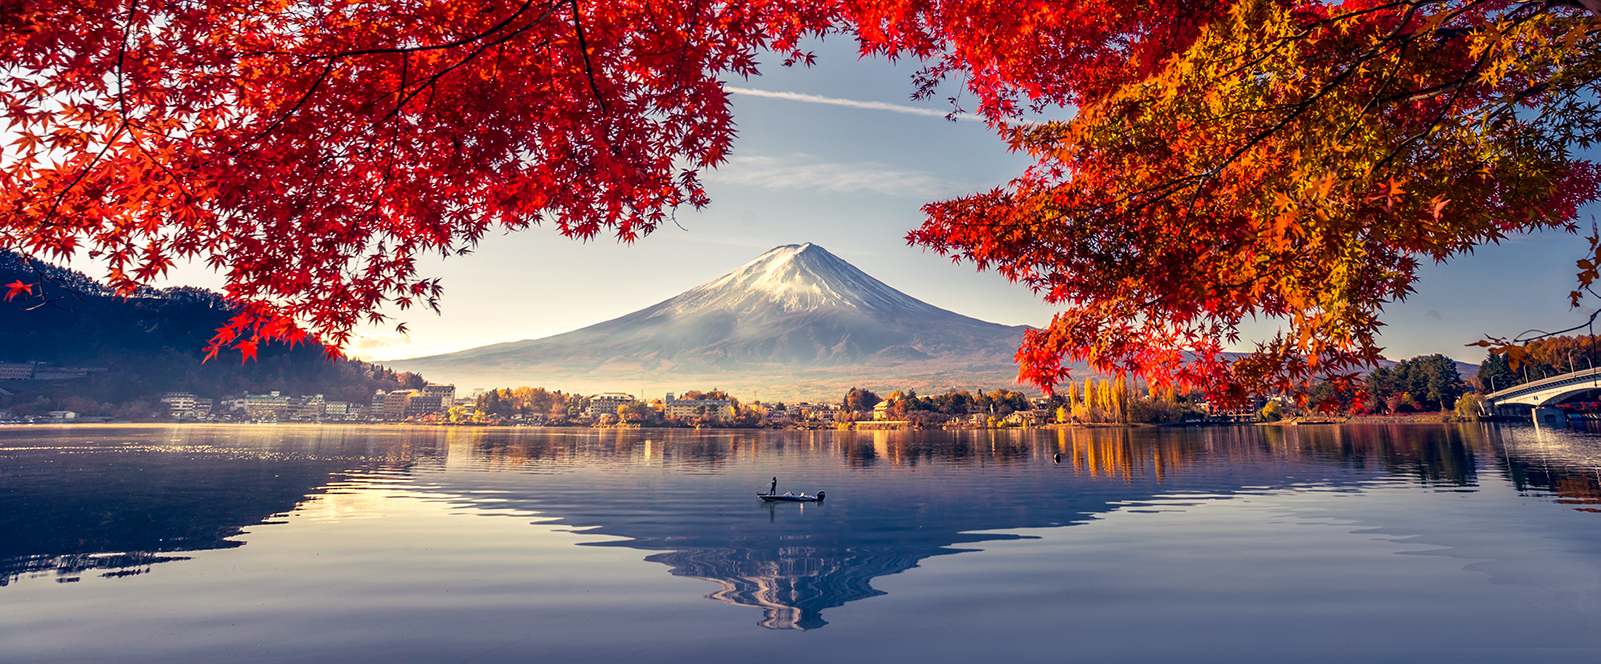
\includegraphics[width=0.7\linewidth]{./Graphics/BeautifulPicture.jpg}
             \caption{This is How you add a beautiful picture}
                \label{BFigure1} %You can use this to refer to this pic
            \end{figure}
            \end{center}
        \end{minipage}
        See the code to check how i referred to this Figure \ref{BFigure1} and upload all your pictures in Graphics folder to create no messy main folder.
\end{frame}
\begin{frame}{函数型数据背景}
        \begin{minipage}[t]{\linewidth}
            \begin{center}
            \begin{figure}
                \centering
                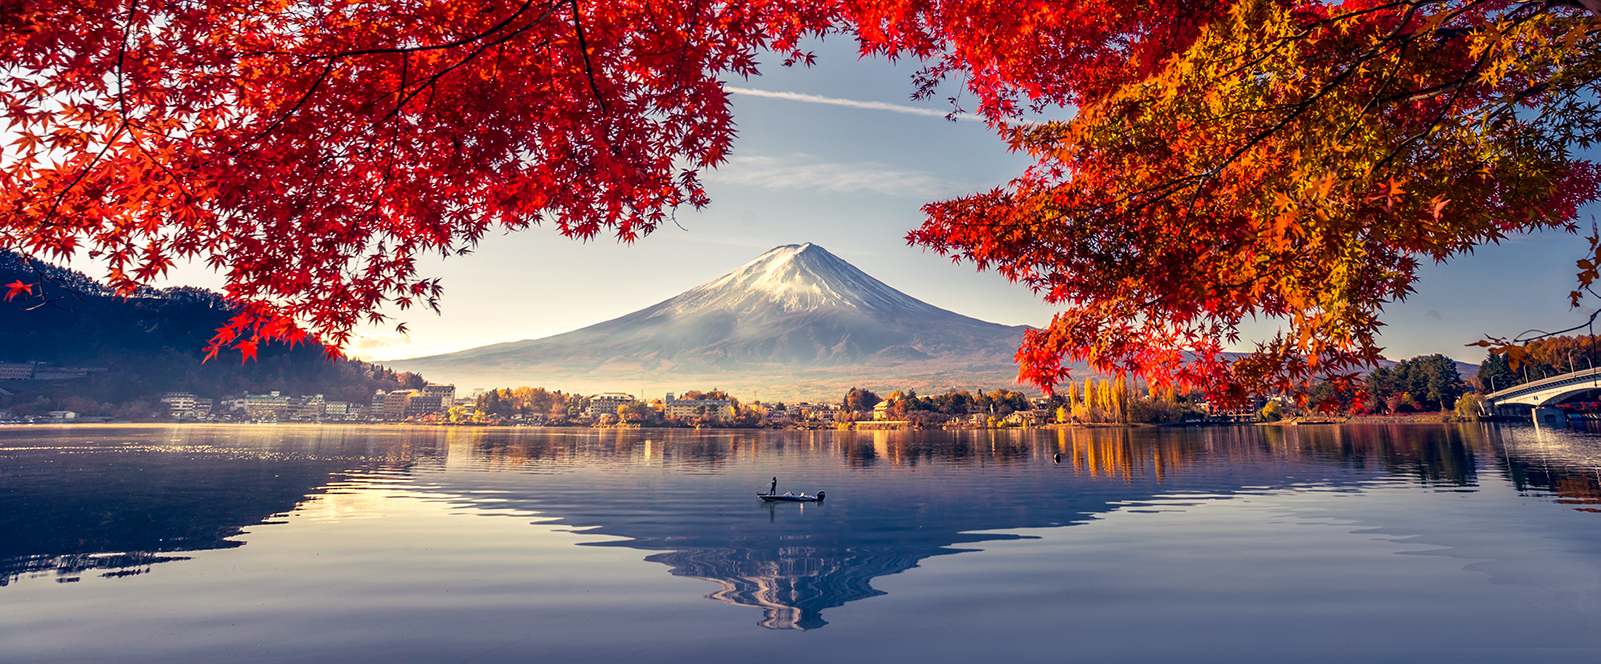
\includegraphics[width=0.7\linewidth]{./Graphics/BeautifulPicture.jpg}
             \caption{This is How you add a beautiful picture}
                \label{BFigure1} %You can use this to refer to this pic
            \end{figure}
            \end{center}
        \end{minipage}
        See the code to check how i referred to this Figure \ref{BFigure1} and upload all your pictures in Graphics folder to create no messy main folder.
\end{frame}
\subsection{为什么对函数型数据的分析很重要?}
\begin{frame}{为什么对函数型数据的分析很重要?}
        \begin{minipage}[t]{\linewidth}
            \begin{center}
            \begin{figure}
                \centering
                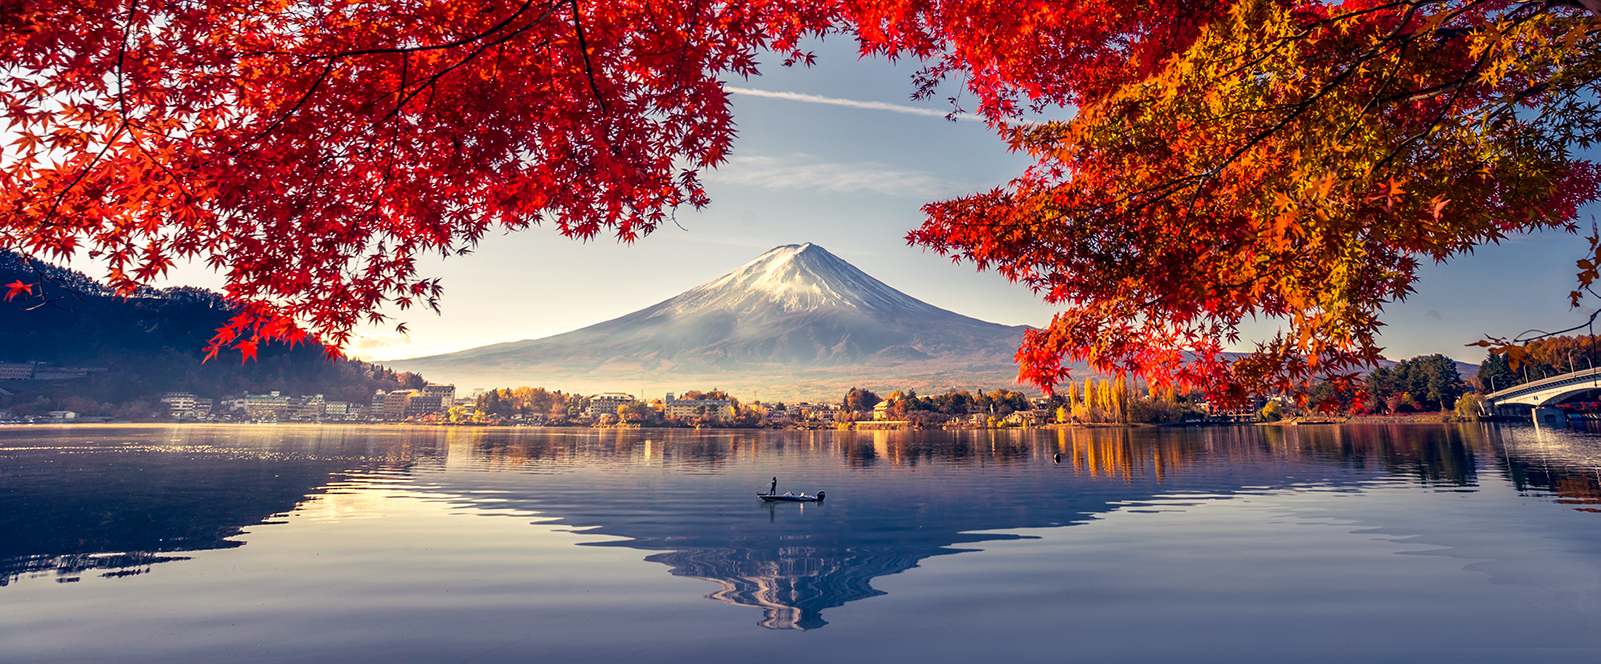
\includegraphics[width=0.7\linewidth]{./Graphics/BeautifulPicture.jpg}
             \caption{This is How you add a beautiful picture}
                \label{BFigure1} %You can use this to refer to this pic
            \end{figure}
            \end{center}
        \end{minipage}
        See the code to check how i referred to this Figure \ref{BFigure1} and upload all your pictures in Graphics folder to create no messy main folder.
\end{frame}
\begin{frame}{为什么对函数型数据的分析很重要?}
        \begin{minipage}[t]{\linewidth}
            \begin{center}
            \begin{figure}
                \centering
                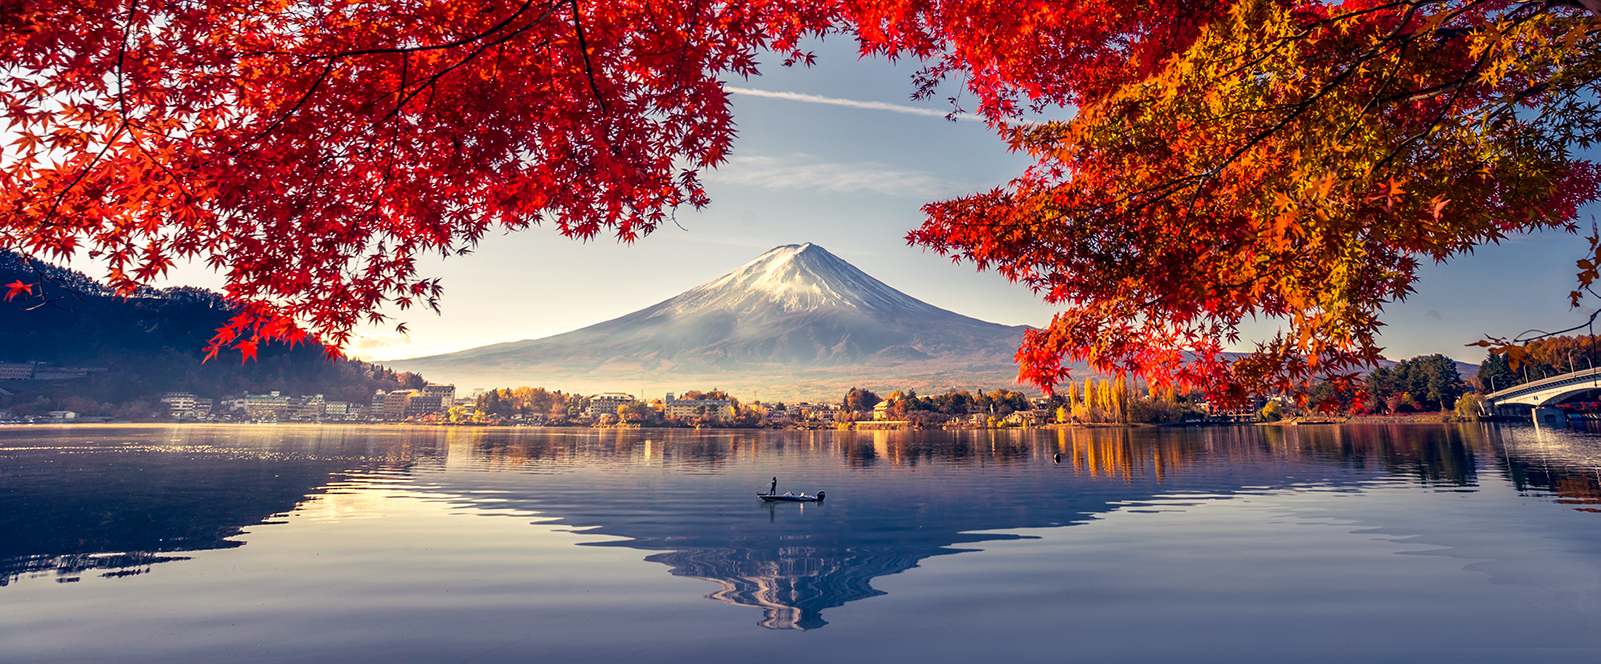
\includegraphics[width=0.7\linewidth]{./Graphics/BeautifulPicture.jpg}
             \caption{This is How you add a beautiful picture}
                \label{BFigure1} %You can use this to refer to this pic
            \end{figure}
            \end{center}
        \end{minipage}
        See the code to check how i referred to this Figure \ref{BFigure1} and upload all your pictures in Graphics folder to create no messy main folder.
\end{frame}


















% 第二部分
\section{论文框架及主要内容}
\subsection{论文框架}
\begin{frame}{论文框架}
    \begin{itemize}
     \setlength{\itemsep}{10pt}
        \item Item 1
        \begin{itemize}
            \item Item 1 Subitem 1
            \item Item 1 Subitem 2
            \item Item 1 Subitem 3
        \end{itemize}
        \item Item 2
        \begin{itemize}
            \item Subitem 1
            \begin{itemize}
                \item Subsubitem 1
            \end{itemize}
            \item Subitem 2
            \begin{itemize}
                \item This is marked subitem \\
                This is unmarked subitem
            \end{itemize}
        \end{itemize}
    \end{itemize}
\end{frame}

\subsection{简要介绍一些观点}
\subsubsection{观点:降维}
\subsubsection{观点:回归}
\subsubsection{观点:聚类}
\subsubsection{新颖的工具}











% 第三部分
\section{一点思考}
\subsection{似乎存在的问题}
\subsection{如何应用}












% 第四部分
\section{总结与展望}








% 一些模板,可自行查看
\begin{frame}{Section 1 Subsection 1: Itemizing Part 1}
    \begin{itemize}
     \setlength{\itemsep}{10pt}
        \item Item 1
        \begin{itemize}
            \item Item 1 Subitem 1
            \item Item 1 Subitem 2
            \item Item 1 Subitem 3
        \end{itemize}
        \item Item 2
        \begin{itemize}
            \item Subitem 1
            \begin{itemize}
                \item Subsubitem 1
            \end{itemize}
            \item Subitem 2
            \begin{itemize}
                \item This is marked subitem \\
                This is unmarked subitem
            \end{itemize}
        \end{itemize}
    \end{itemize}
\end{frame}



\begin{frame}{Section 2 Subsection 2: Itemizing Part 2}
\begin{itemize}
    \item[Step 1] This is step 1
    \item[Step 2] This is step 2
    \item[Step 3] Yuo can add small equation in text $y=mx+c$ or $x^{3}=2y$
    \item[Step 4] You can add a separate equation
        \begin{align*}
        |\Psi \rangle = \sum_{i} u_{i} | \varphi_{i} \rangle 
    \end{align*}
\end{itemize}
\end{frame}




\begin{frame}{Section 1 Subsection 3: Footnote Citing}
\begin{itemize}
    \item This is simple text
    \item This text is footnote cited \footnotemark
    \item Add you resources in bibliography file 
\end{itemize}
        \footnotetext{\cite{AmorphousGraphene}}
\end{frame}




\begin{frame}{Section 2 Subsection 2: Equation}
    \begin{flushleft}
    \textbf{Name of Some Theorem}
    \end{flushleft} 
    \begin{align}
         \Psi (\Vec{r}+ \Vec{R}) = e^{i\Vec{k}\cdot\Vec{R}}\Psi(\Vec{r})
    \end{align}
    Where
    \begin{itemize}
        \item $\Vec{R}$ is somethin
        \item $\Vec{k}$ is something
    \end{itemize}
\end{frame}



\begin{frame}{Section 2 Subsection 3: Multiple Equations}
    \begin{align}
        |\Psi \rangle = \frac{1}{\sqrt{N}} \sum_{i}^{N} e^{i\Vec{k}\cdot\Vec{R}_{i}}|s_{i}\rangle \label{Wavefunc} \\ 
        \frac{1}{\sqrt{N}} \sum_{j=1}^{N} \left[ H_{ij}e^{i\Vec{k}\cdot\Vec{R}_{j}}-\varepsilon e^{i\Vec{k}\cdot\Vec{R}_{i}}\right] = 0 \label{Eq0003}
    \end{align}
    As you can see in equation \ref{Eq0003}. Chcek how i referred to this equation in code. 
\end{frame}



\begin{frame}{Add Picture or Figure}
        \begin{minipage}[t]{\linewidth}
            \begin{center}
            \begin{figure}
                \centering
                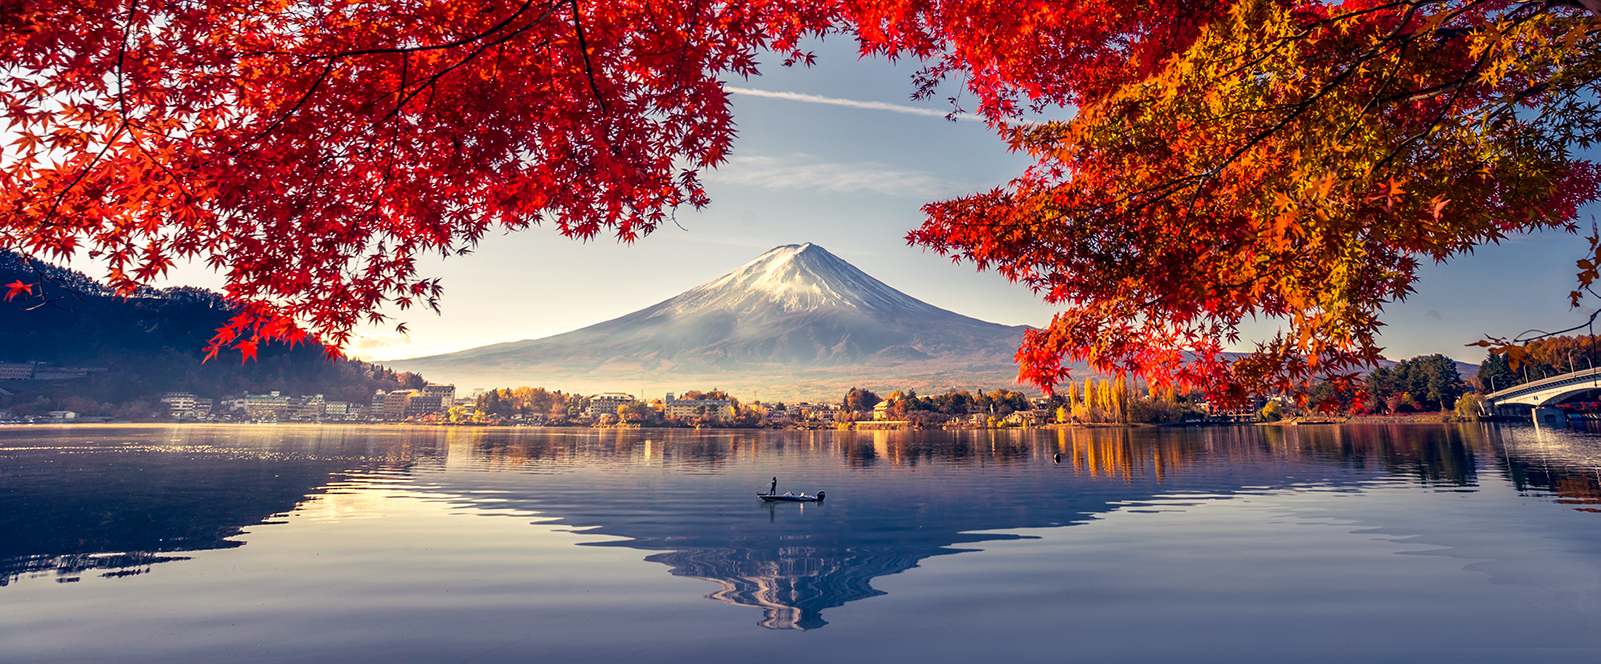
\includegraphics[width=0.7\linewidth]{./Graphics/BeautifulPicture.jpg}
             \caption{This is How you add a beautiful picture}
                \label{BFigure1} %You can use this to refer to this pic
            \end{figure}
            \end{center}
        \end{minipage}
        See the code to check how i referred to this Figure \ref{BFigure1} and upload all your pictures in Graphics folder to create no messy main folder.
\end{frame}

% 取消下列注释可以得到引文目录
%\section*{References}
%\begin{frame}{References}
%\bibliographystyle{IEEEtranN}
%\bibliography{bibliography.bib}
%\end{frame}
\end{document}